\section{Applications}

Design the following applications and provide APIs to users.

\subsection{Routing protocol}
\iffalse
\begin{figure}[htbp]
	\centering
	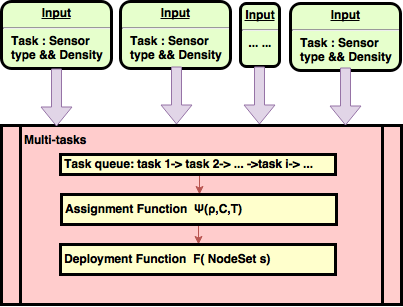
\includegraphics[width=2in]{Figure/Multi-tasks}
	\caption{Multi-tasks.}
	\label{system}
\end{figure}
\fi

\iffalse
\subsection{Evaluator}
\iffalse
\begin{figure}[htbp]
	\centering
	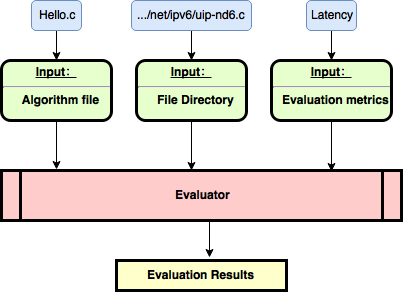
\includegraphics[width=2in]{Figure/Evaluator}
	\caption{Evaluator.}
	\label{system}
\end{figure}
\fi
Provide APIs for users to update network algorithms through OTA.
\begin{itemize}
\item[Input:] the algorithm function and its location/standard name(tell where to replace it) 
\end{itemize}

Evaluate the performance of the new algorithm.
\begin{itemize}
\item[Input:] the evaluation metrics
\end{itemize}

In our implementation, we will take neighbor discovery algorithms for experiments.
\fi



\subsection{Node selection}

AI helps creating smarter sensor systems.

AI systems have been improving, and new advances in machine intelligence are creating seamless interactions between people and digital sensor systems.

 In sensor systems, applications can be found for a variety of tasks, including selection of sensor inputs, interpreting signals, condition monitoring, fault diagnosis, machine and process control, machine design, process planning, production scheduling, and system configuring. Some examples of specific tasks undertaken by expert systems are:
* Assembly 
* Automatic programming 
* Controlling intelligent complex vehicles  
* Planning inspection 
* Predicting risk of disease 
* Selecting tools and machining strategies 
* Sequence planning 
* Controlling plant growth. 

AI can increase effective communication, reduce mistakes, minimize errors, and extend sensor life.



The tools and methods described have minimal computation complexity and can be implemented on small assembly lines, single robots, or systems with low-capability microcontrollers. These novel approaches proposed use ambient intelligence and the mixing of different AI tools in an effort to use the best of each technology. The concepts are generically applicable across many processes.


minimum energy, data loss, reliability, robustness, etc., in place during the design and operation of wireless sensor networks

a specific set of protocols for medium access, localization and positioning, time synchronization, topology control, security and routing are identified based on the current configuration of the network, the requirements of the application and the topology of their deployment.

\subsection{Task scheduler}

Each task has a deployment density $\rho$.

Assign tasks to the sensors with less tasks first.

Assign tasks to critical nodes fitst

\subsection{Network monitoring and visualization}

Visualize network monitoring and monitor the network in real-time.

Make the system user-friendly(easy to use).
